%%%%%%%%%%%%%%%%%%%%%%%%%%%%%%%%%%%%%%%%%%%%%%%%
\section{Tips}


%%%%%%%%%%%%%%%%%%%%%%%%%%%%%%%%%%%%%%%%%%%%%%%%%%%%%%%
\begin{frame}

\frametitle{Building a workflow}

\begin{enumerate}
  \item I ``looked down'' on {\texttt{bash}} scripts before, but you might want to start from that on one data file first as a starting point.  Convert this to a Snakemake file.
  \item Because of how wildcards are carried backwards (i.e., the {\green{corpus}} variable), you might want to start connecting things up from the {\magenta{all}} rule.
  \item The Linux {\texttt{touch}} command can be useful here.  It updates the date/time or creates a new file with 0 bytes with the current date and time.
    \begin{itemize}
      \item So, you can link up the workflow first with {\texttt{touch \{output\}}} and then write the actual commands afterwards.
    \end{itemize}
  \item I started {\red{numbering}} my output directories to help me figure out the order of the output files.
  \item Send error messages of programs to the {\blue{log}} directive.  If a rule fails, then you have a message to read.
\end{enumerate}

\end{frame}


%%%%%%%%%%%%%%%%%%%%%%%%%%%%%%%%%%%%%%%%%%%%%%%%%%%%%%%
\begin{frame}

\frametitle{Testing a workflow}

Use:
\begin{itemize}
  \item a small test file.
  \item a single core ({\texttt{--cores 1}}) when testing.  With more cores, the rules are executed simultaneously.  Thus, the output will interleave and you can't tell which rule output what!
  \item the {\texttt{-p}} option so that it prints the command that it is running.
\end{itemize}

\end{frame}


%%%%%%%%%%%%%%%%%%%%%%%%%%%%%%%%%%%%%%%%%%%%%%%%%%%%%%%
\begin{frame}

\frametitle{Debugging a workflow}

\begin{figure}
  \centering
  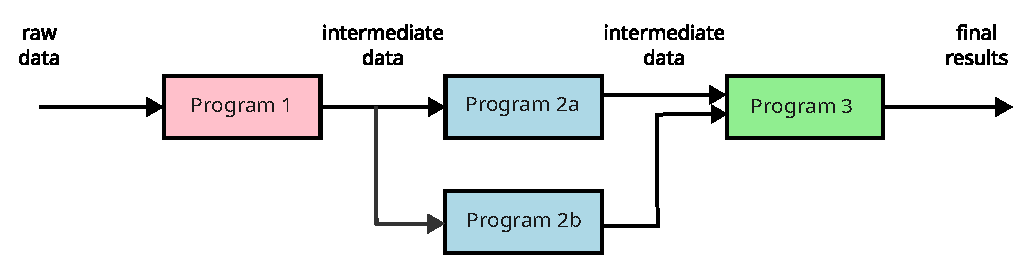
\includegraphics[width=\linewidth]{tips/pipeline-example-branching.eps}
\end{figure}

When trying to find out where in your workflow is causing you grief, you can remove an entire branch by commenting it out from the {\green{input}} directive of the rule it is going to.
\vs

Snakemake seems to:
\begin{enumerate}
  \item Start from the end to the beginning, looking for which paths to follow.
  \item When the execution paths are known, it runs it in the forward direction from the beginning.
\end{enumerate}

\end{frame}


%%%%%%%%%%%%%%%%%%%%%%%%%%%%%%%%%%%%%%%%%%%%%%%%%%%%%%%
\begin{frame}

\frametitle{Common error message}

\begin{figure}
{\fbox{
  \begin{tabularx}{\linewidth}{X}
IncompleteFilesException:\\
The files below seem to be incomplete. If you are sure that certain files are not incomplete, mark them as complete with\\
\\
{\D\D}snakemake --cleanup-metadata <filenames>\\
\\
To re-generate the files rerun your command with the --rerun-incomplete flag.  Incomplete files:\\
...\\
\end{tabularx}
}}
\end{figure}
\vs

Snakemake stores its progress in a run in a ``hidden'' directory called {\red{\texttt{.snakemake}}}.  If it starts getting its state wrong (i.e., you think it completed its last run, but it does not think so), then delete this directory and all of the output.  Then, start again.

\end{frame}
